\section{Datalaag}
De applicatie bevat data uit verschillende bronnen, en slaat zijn data in verschillende bronnen op. Deze data en de verbindingen met de bronnen vormen de datalaag.

\subsection{Ruwe inkomende data}

De transponderleverancier \mylaps heeft een SDK beschikbaar gesteld aan Emando, waarmee het mogelijk is om de doorkomsten van transponders realtime binnen te krijgen. Om deze databron te benaderen bevat de datalaag een Data Collector, geïmplementeerd als Azure Cloud Worker Role, welke non-stop draait op één cloud instance. Dit proces onderhoudt de verbinding met de \mylaps SDK.

Vanuit de \mylaps SDK ontvangt de data laag realtime de doorkomsten van iedere transponder die langs een lus komt. Deze doorkomsten bevatten een tijdstip, een transpondernummer en een plaats op de baan. Zodra een van deze doorkomsten binnen komt, wordt deze direct opgeslagen voor toekomstig gebruik in een doorkomstentabel in Azure Table Storage. Het kan namelijk voorkomen dat de transponder van de zojuist binnengekomen doorkomst nog niet gekoppeld is aan een gebruikersaccount. Wanneer dit het geval is, kunnen er (nog) geen aggregaties uitgevoerd worden op deze data.

\begin{figure}[ht]
  \begin{center}
  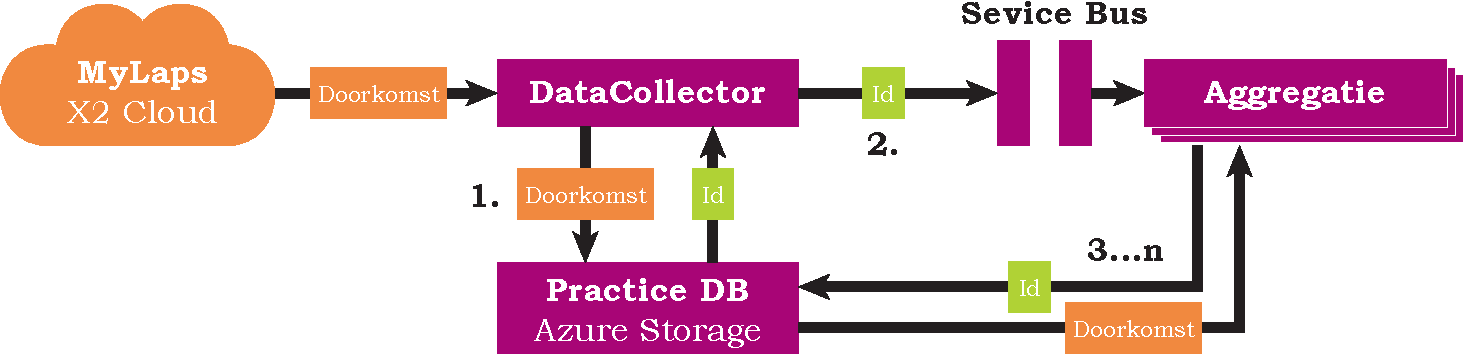
\includegraphics[width=\textwidth]{style/images/datacollector-flow}    
  \end{center}
  \caption{De werking van de Data Collector en de Service Bus}
  \label{fig:datacollector}
\end{figure}

Door deze data op te slaan, is het mogelijk om later functionaliteit in te bouwen om alsnog over deze data te kunnen aggregeren.

Nadat de data opgeslagen is, wordt via een Azure Service Bus het Id van de doorkomst doorgestuurt naar het aggregatieproces in de businesslaag. Het aggregatieproces raadpleegt bij het binnenkrijgen van dit Id opnieuw de doorkomst, om zo minder data over de zogenaamde service bus te versturen en altijd over up to date data te beschikken. Dit process wordt weergegeven in figuur~\ref{fig:datacollector}.

\subsection{Entiteiten}
In figuur~\ref{fig:entiteiten} wordt een deel van de entiteiten die de applicatie gebruikt getoond, inclusief de onderlinge relaties. De entiteiten die te maken hebben met externe data en accounts worden opgeslagen met behulp van Azure SQL, zoals ook besproken in sectie~\ref{sec:database} van het oriëntatieverslag. De entiteiten die te maken hebben met doorkomsten en aggregaties worden opgeslagen in Azure Table Storage.

\begin{figure}[ht]
  \begin{center}
  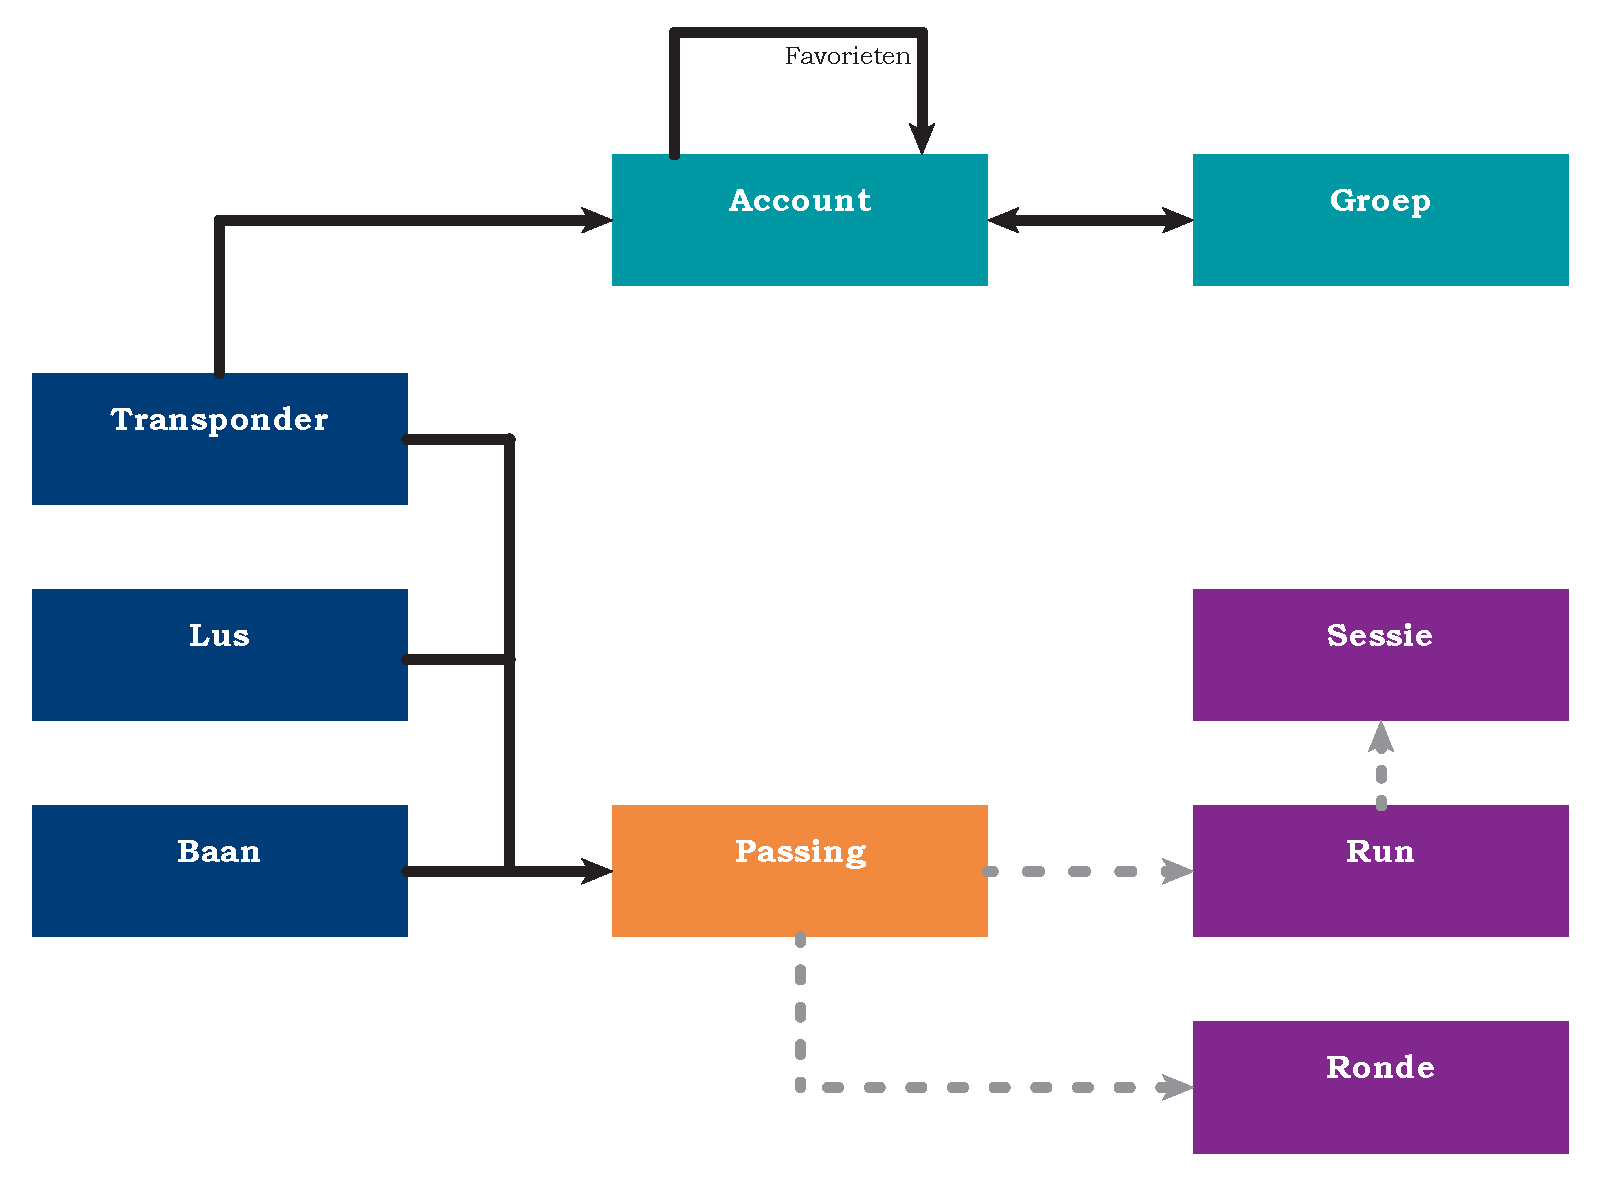
\includegraphics[width=.9\textwidth]{style/images/Entiteiten}    
  \end{center}
  \caption{De entiteiten en hun relaties.}
  \label{fig:entiteiten}
\end{figure}

Hoewel de daadwerkelijke structuur van de data in Azure Table Storage anders is dan in de figuur, geeft de figuur toch een goed beeld van deze entiteiten en hun relaties. 

\subsection{Azure SQL \& Entity Framework}
Azure SQL is de relationele SQL database van Azure en omdat de relaties in onze entiteiten worden beschreven door het Entity Framework~\cite{entityframework-msdn, entityframework-facto}, gebruikt onze applicatie de Entity Framework driver voor Azure SQL. Entity Framework is de de facto standaard voor relationele datalagen in ASP.NET. Het kan bijvoorbeeld relaties tussen entiteiten automatisch opzoeken. Ook hoeft geen SQL code geschreven te worden. Om entiteiten op te kan kan platformonafhankelijke LINQ code geschreven worden.

\subsection{Azure Table Storage}
De geaggregeerde data kan ``plat'' worden opgeslagen met behulp van NoSQL. Door alleen passings (doorkomsten), rondes en leaderboard-waarden entiteiten op te slaan in de aggregatiedatabase, hoeven onderlinge relaties niet bijgehouden te worden en kunnen gegevens goedkoop opgevraagd worden. Gegevens zoals ``rust/run''-ronde en sessies zijn onderdeel van rondes. De snelheid en segmenten worden niet opgeslagen, maar direct verstuurd naar de applicatie.

Vanuit Emando ging de voorkeur voor het opslaan van de geaggregeerde data  uit naar de NoSQL Azure Table Storage. De Azure Table Storage integreert eenvoudig met de reeds bestaande infrastructuur van het bedrijf. Bovendien biedt een gepartitioneerde en gesorteerde Azure Table Storage tabel een groot performancevoordeel: het goedkoop en snel kunnen selecteren van de laatste entiteiten per context.

Bij het gebruik van NoSQL is het belangrijk dat de Partition- en Row Key efficiënt gekozen worden, aangezien dit de snelheid van het zoeken bepaalt. Verder is het belangrijk dat de combinatie van Partition en Row Key uniek is. In figuren \ref{fig:passingTableStructure}, \ref{fig:userPassingTableStructure}, \ref{fig:lapTableStructure} en \ref{fig:lapLeaderboardTableStructure} is te zien hoe deze keys gekozen zijn en wat de structuur van deze tabellen is.

Vanuit de Data Collector worden de doorkomsten die realtime binnen komen opgeslagen in Azure Table Storage als backup. De structuur van deze tabel is terug te vinden in figuur \ref{fig:passingTableStructure}. Verderop in het aggregatieproces worden deze doorkomsten gekoppeld aan gebruikers. Deze aggregaties worden vervolgens opgeslagen in een aparte tabel binnen Azure Table Storage. De structuur van deze tabel is terug te vinden in figuur \ref{fig:userPassingTableStructure}.

Verderop in het aggregatieproces worden doorkomsten van gebruikers gekoppeld aan sessies, rondes en run/rust periodes. Deze aggregaties worden opgeslagen in de rondetabel binnen Azure Table Storage. De structuur hiervan is terug te vinden in figuur \ref{fig:lapTableStructure}.

Van snelheden, rondes, run/rust periodes en sessies worden leaderboards bijgehouden in Azure Table Storage. Deze hebben elk een eigen corresponderende tabel, zodat aggregaties parallel aan elkaar leaderboards kunnen updaten.
Alle leaderboards zijn voorzien van een leaderboard Id en een user Id. Het leaderboard Id houdt bij voor welke context het leaderboard geldig is. Dit kunnen banen, groepen, maar ook gebruikers zijn. Wanneer een gebruiker een ronde rijdt op een baan X, moeten zijn records voor de baan, zijn groepen en zijn eigen totalen geüpdatet worden. Een voorbeeldstructuur van deze leaderboards is te vinden in figuur \ref{fig:lapLeaderboardTableStructure}.

\begin{figure}[h!]
  \begin{center}
  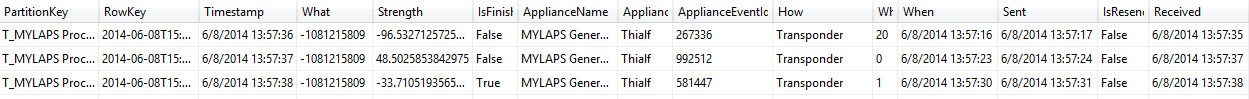
\includegraphics[width=\textwidth]{style/images/passingsStructure}    
  \end{center}
  \caption{De doorkomstentabel met voorbeeld records. Doorkomsten bevatten 2 kernelementen, waar op gefilterd wordt: e transponder (bestaande uit een type en een nummer) en het tijdstip waarin de doorkomst binnen kwam. Door de keys als volgt in te richten kan daarom efficiënt gezocht worden binnen de data: de Partition Key is het type transponder + transpondernummer en de Row Key het tijdstip waarop de doorkomst binnen kwam.}
  \label{fig:passingTableStructure}
\end{figure}

\begin{figure}[h!]
  \begin{center}
  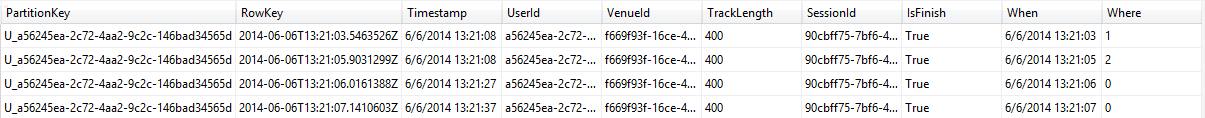
\includegraphics[width=\textwidth]{style/images/userPassingsStructure}    
  \end{center}
  \caption{De doorkomstentabel met voorbeeldrecords. Gebruikers doorkomsten bevatten 2 kernelementen, waar op gefilterd wordt: de gebruiker en het tijdstip waarin de doorkomst binnen kwam. Door de keys als volgt in te richten kan daarom efficiënt gezocht worden binnen de data: de Partition Key is het account Id \\met een prefix voor gebruikers en de Row Key het tijdstip waarop de doorkomst binnen kwam.}
  \label{fig:userPassingTableStructure}
\end{figure}

\begin{figure}[h!]
  \begin{center}
  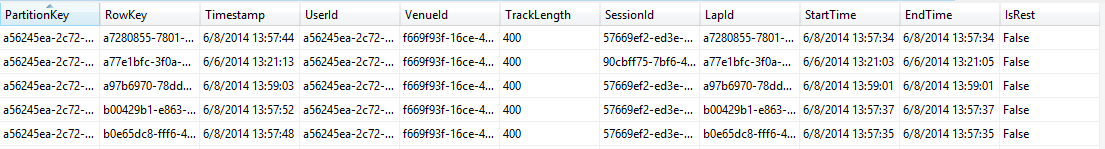
\includegraphics[width=\textwidth]{style/images/aggregationLapsStructure}    
  \end{center}
  \caption{De rondetabel met voorbeeldrecords. Gebruikersdoorkomsten bevatten 2 kernelementen, waar op gefilterd wordt: de gebruiker en het rondenummer zelf. Door de keys als volgt in te richten kan daarom efficiënt gezocht worden binnen de data: de Partition Key is het account Id en de Row Key het ronde Id.}
  \label{fig:lapTableStructure}
\end{figure}

\begin{figure}[h!]
  \begin{center}
  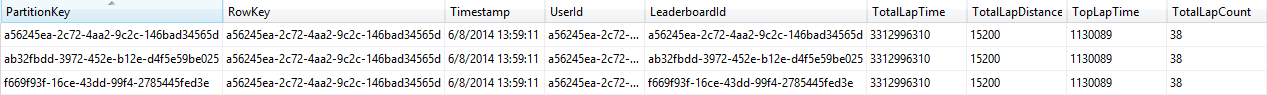
\includegraphics[width=\textwidth]{style/images/lapLeaderboardStructure}    
  \end{center}
  \caption{De ronde-leaderboardtabel, een voorbeeld van een leaderboardtabel. Leaderboards bevatten 2 kernelementen, waar op gefilterd wordt: de gebruiker en de context waar het leaderboard voor is (groep, baan of gebruiker). Door de keys als volgt in te richten kan daarom efficiënt gezocht worden binnen de data: de Partition Key het account Id\\ en de Row Key het context Id (groep, baan of account Id).}
  \label{fig:lapLeaderboardTableStructure}
\end{figure}

\clearpage
